\documentclass[a4paper, 12pt]{article}
\usepackage[utf8]{inputenc}
\usepackage[T1]{fontenc}
\usepackage[french]{babel}
\usepackage{graphicx}
\usepackage{amsmath}
\usepackage{hyperref}
\usepackage{lmodern}
\usepackage{moreverb}
\usepackage{multicol}

\hypersetup{
    colorlinks=true,
    linkcolor=blue,
    filecolor=magenta,      
    urlcolor=cyan,
    pdftitle={Overleaf Example},
    pdfpagemode=FullScreen,
    }

\urlstyle{same}
\usepackage[a4paper,left=2cm,right=2cm,top=2cm,bottom=2cm]{geometry}

\pagestyle{headings}
\pagestyle{plain}


\setcounter{secnumdepth}{4}
\setcounter{tocdepth}{4}
\makeatletter

\makeatother

\makeatletter
\def\toclevel@subsubsubsection{4}
\def\toclevel@paragraph{5}
\def\toclevel@subparagraph{6}
\makeatother


\setlength{\parindent}{0cm}
\setlength{\parskip}{1ex plus 0.5ex minus 0.2ex}
\newcommand{\hsp}{\hspace{20pt}}
\newcommand{\HRule}{\rule{\linewidth}{0.5mm}}

\begin{document}

\begin{titlepage}
  \begin{sffamily}
  \begin{center}

   
    \textsc{\LARGE }\\[2cm]

    \textsc{\Large Compte rendu de Réunion}\\[1.5cm]
    \textsc{\Medium Rédigé par BENGUEZZOU Idriss}

    % Title
    \HRule \\[0.4cm]
    { \huge  \textsc{StellaStone} \\
    \textsc{\Large By Novus}\\ [0.4cm] }
	

    \HRule \\[2cm]
    \textsc {Idriss BENGUEZZOU\\Mohammed ROUABAH\\Ghilas MEZIANE \\ Ilyes ZEGHDALLOU}
 \begin{figure}
     \centering
    
\includegraphics[scale=0.2]{logoUJM.png}
     \label{fig:ujm_logo}
 \end{figure}
   
    \

    \vfill

    % Bottom of the page
    {\large {} 28/11/2022}

  \end{center}
  \end{sffamily}
\end{titlepage}

\newpage

\section{Réunion du Vendredi 25/11}
La réunion de cette semaine a eu lieu le vendredi 25 novembre 2022, en présentiel sur le créneau horaire 18h00-19h00 sur notre serveur Discord.
Celle-ci s'est tenue en présence de tous les membres du groupe.

\textbf{Ordre du jour :}

\begin{itemize}
    \item Relecture du documents de spécifications des exigences.
    \item Observation de l'avancement du document de conception générale.
    \item Observation de l'avancement du document de tests de recette.
    \item Introduction au document manuel Utilisateur.
\end{itemize}

\section{Tour de table habituel}


Mr.BENGUEZZOU Idriss et Mr.MEZIANE Ghilas ont achevé le document de spécification des exigences. \\ 
Mr.ROUABAH et Mr.ZEGHDALLOU ont pris du retard sur le documents tests de recette, c'est pourquoi Mr.BENGUEZZOU et Mr.MEZIANE ont pris le relais laissant ainsi Mr.ROUABAH et Mr.ZEGHDALLOU continuer leur avancée sur le document de conception générale.

De plus, en se référant au diagramme de Gantt, Mr.BENGUEZZOU a rappelé à l'ensemble du groupe qu'il était prévu de faire relire le document de spécification des exigences par une autre entreprise.

\section{Introduction au manuel utilisateur}
Durant la réunion, nous avons eu l'occasion de retracer les objectifs pour le document "manuel utilisateur". Nous nous sommes aidés de ressources trouvées sur Internet dont voici un exemple:
\href{https://apps.who.int/iris/bitstream/handle/10665/205234/9789242500196_software_fre.pdf}{Manuel utilisateur - WISN - OMS}
Nous nous servirons de cet exemple parmi tant d'autres pour la rédaction afin de structurer notre document et faciliter sa rédaction.
\section{Décisions prises}
\begin{itemize}
    \item Organiser une réunion avec le groupe GMAO, afin de relire nos documents respectifs le 28/11/2022 sur le créneau horaire 21h30 - 00h00.
    \item Mise à jour du diagramme de Gantt et modification des dates butoirs.
\end{itemize}

\newpage
\section{Révision du planning}

 \begin{figure}[!h]
    \centering
    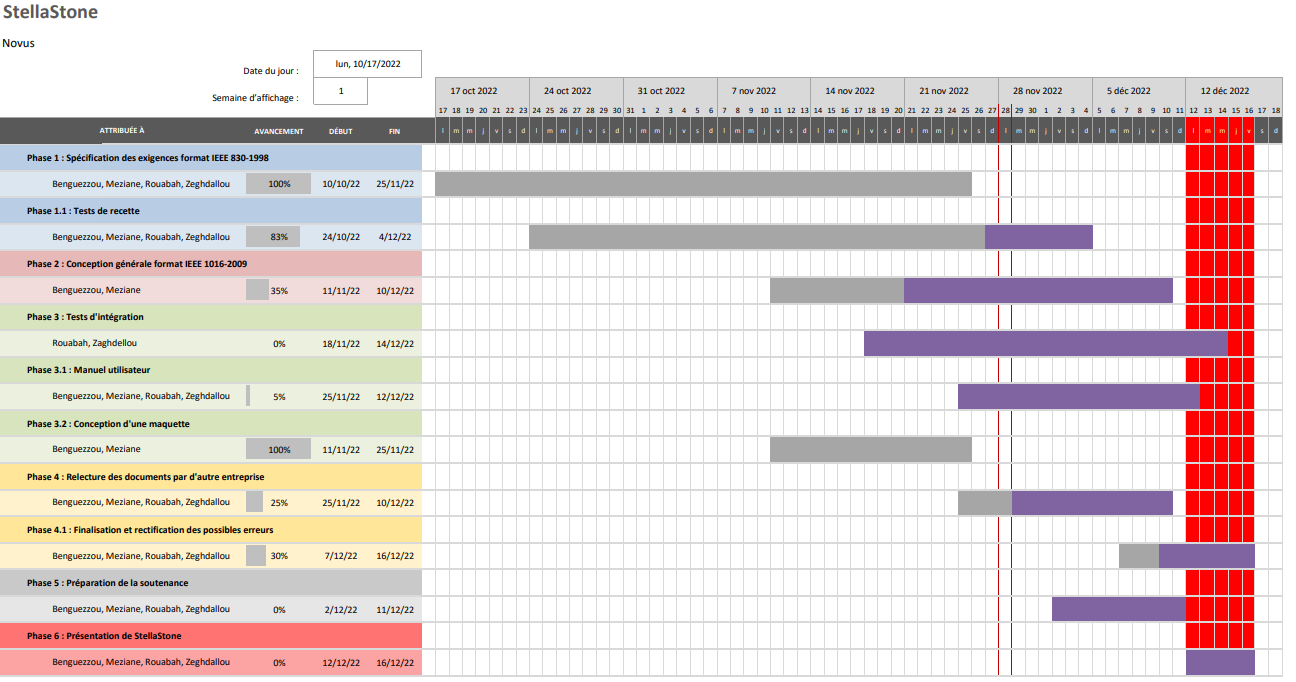
\includegraphics[scale=0.45]{diagramme.png}
    \label{fig:Le_planning}
    \caption{Diagramme de Gantt}
\end{figure}
\section{Prochaine réunion et objectifs de la semaine}
Comme objectifs de la semaine, Mr.BENGUEZZOU et Mr.MEZIANE devront finaliser le document de tests de recette et s'atteler à la rédaction du manuel utilisateur. 

Mr.ROUABAH et Mr.ZEGHDALLOU seront tenus de continuer le document de conception générale et de commencer la rédaction des tests d'intégration.

La prochaine réunion qui devait être fixée au 3 décembre n'aura finalement pas lieu compte tenu de la densité de travail que nous devons fournir cette semaine. Néanmoins des réunions informelles auront lieu tout au long de la semaine, selon les disponibilités des chacun afin de mener à bien la rédaction de tous les documents demandés. Ainsi la prochaine réunion aura lieu le 09 décembre 2022 sur le créneau horaire 19h-20h.

\end{document}